
\subsection{Erasure Coding}
\label{sec:ec_background}

It has been known that failures in storage systems are common \cite{ghemawat03}.
Components in a storage system can fail in numerous ways, including sector
errors, bit flips and physical failures \cite{plank13}. Erasure coding provides
redundancy to prevent data loss in an event of component failure. Here, we
provide the background details of the erasure codes considered in
this work. 

\subsubsection{Replication}

The simplest form of erasure code is replication, in which we make $k$ copies
for each byte in the data and distribute the copies across $k$ devices. As a
result, we can tolerate at most $k-1$ failures as there is at least one
surviving copy for each byte of data.

Although replication is very simple, it introduces high storage overhead. For
example, GFS \cite{ghemawat03} by default tolerates up to two simultaneous
device failures, which requires a storage cost that is $3\times$ that of the original
size of data.

\subsubsection{Maximum Distance Separable Codes}

%We refer readers to the tutorial \cite{plank13} 
%for the essential details of erasure coding in the context of storage systems. 

\begin{figure}[t]
    \centering
    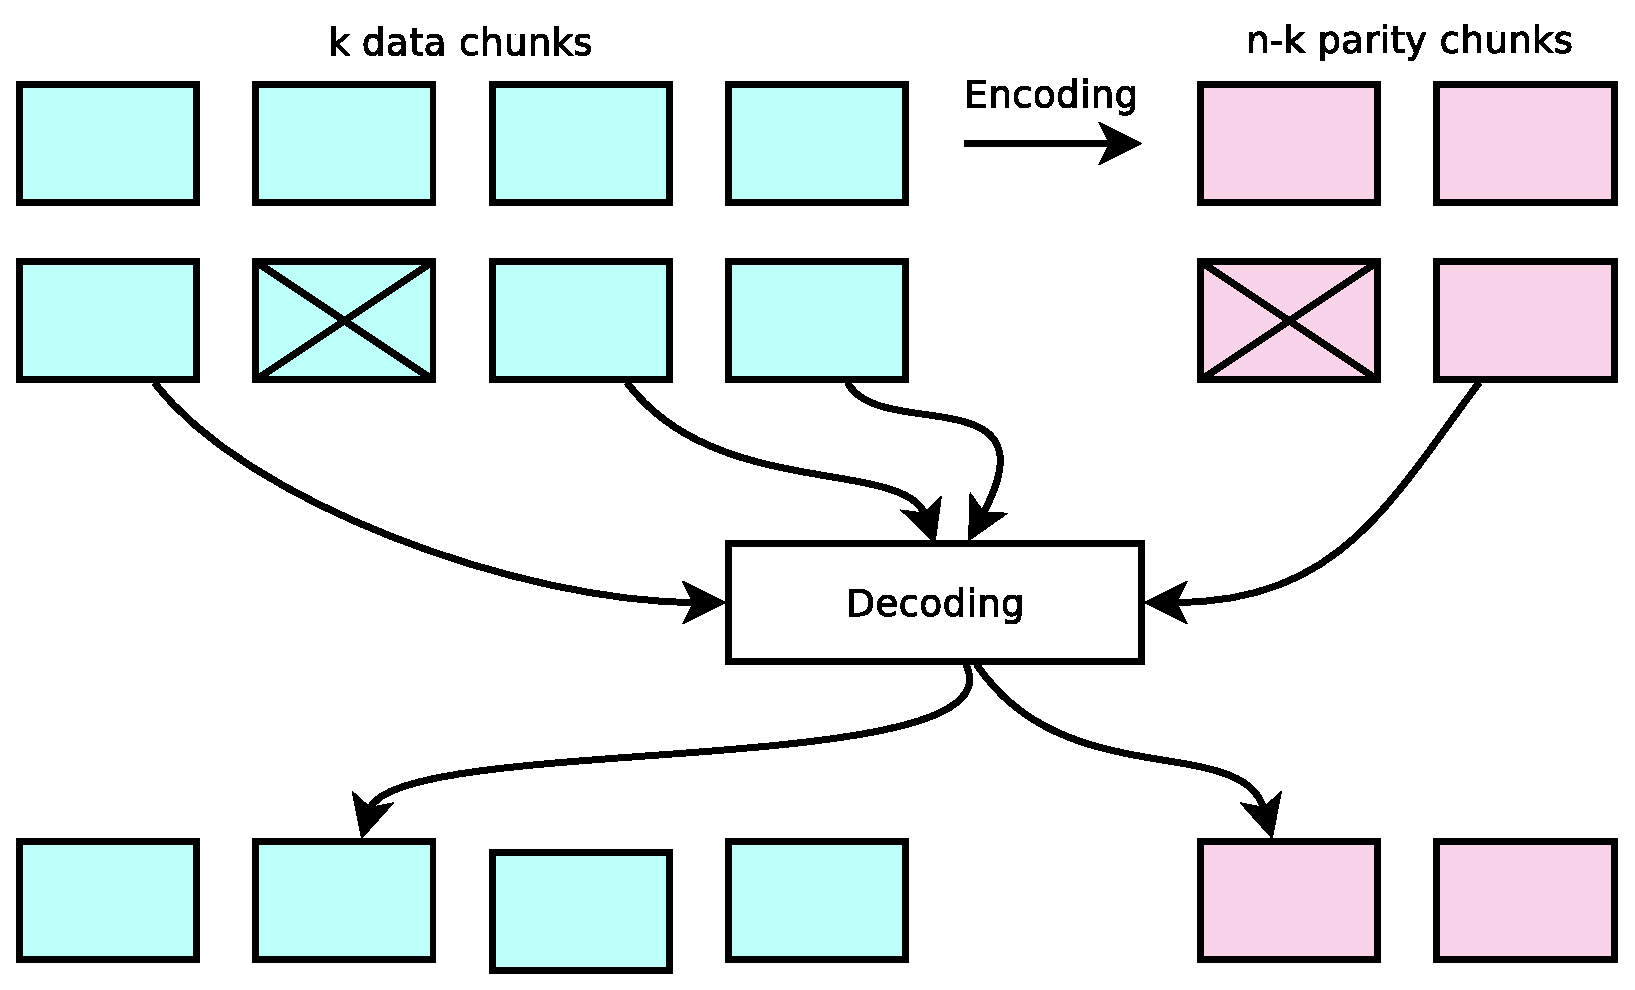
\includegraphics[width=0.7\linewidth]{figs/erasure_code}
    \caption{An $(n,k)$-code encodes $k$ data chunks into $n-k$ parity chunks.
        When up to $n-k$ chunks fail, their content can be recovered using the
        information in the remaining $k$ chunks.}
    \label{fig:erasure_code}
\end{figure}

Figure~\ref{fig:erasure_code} illustrates the acts of encoding and decoding. 
We consider an erasure-coded storage cluster with $M$ nodes (or servers).  We
divide data into {\em segments} and apply erasure coding independently on a
per-segment basis.  We denote an $(n,k)$-code as an erasure coding scheme
defined by two parameters $n$ and $k$, where $k<n$.  An $(n,k)$-code divides a
segment into $k$ equal-size uncoded chunks called {\em data chunks}, and
encodes the data chunks to form $n-k$ coded chunks called {\em parity chunks}.
We assume $n < M$, and have the collection of $n$ data and parity chunks
distributed across $n$ of the $M$ nodes in the storage cluster.  We consider
{\em Maximum Distance Separable (MDS)} erasure codes, i.e., the original segment
can be reconstructed from any $k$ of the $n$ data and parity chunks. 

An MDS code provides optimal fault tolerance for a given storage overhead. For
example, using a $(8,6)$-code can reduce the redundancy overhead to $33\%$,
which is significantly less than $200\%$ in three-way replication, without
sacrificing the level of fault tolerance. 

There are many variants of MDS codes, such as, Reed-Soloman (RS) codes
\cite{reed60}, RDP \cite{corbett04}, EVENODD \cite{plank08} and Liberation
\cite{blaum95}. These codes mainly differ in the ways of calculating the parity chunks.

\subsubsection{Linearity Property of Erasure Codes}

Each parity chunk can be in general encoded by computing a linear combination
of the data chunks.  Mathematically, for an $(n,k)$-code, let
$\br{\gamma_{ij}}_{1\le i\le n-k, 1\le j\le k}$ be a set of encoding
coefficients for encoding the $k$ data chunks $\br{D_1, D_2,\cdots,D_k}$ into
$n-k$ parity chunks $\br{P_1,P_2,\cdots,P_{n-k}}$.  Then, each parity chunk
$P_i$ ($1\le i\le n-k$) can be computed by:
$P_i = \sum_{j=1}^{k} \gamma_{ij} D_j$, 
where all arithmetic operations are performed in the Galois Field over the
coding units called {\em words}. 

The linearity property of erasure coding provides an alternative to computing
new parity chunks when some data chunks are updated.  Suppose that a data
chunk $D_l$ (for some $1\le l\le k$) is updated to another data chunk $D_l'$. 
Then each new parity chunk $P_i'$ ($1\le i\le n-k$) can be computed by:

\begin{equation*}
P_i' = \sum_{j=1,j\ne l}^{k} \gamma_{ij} D_j + \gamma_{il} D_l' 
= P_i + \gamma_{il}(D_l' - D_l). 
\end{equation*}

Thus, instead of summing over all data chunks, we compute new parity chunks
based on the change of data chunks.  The above computation can be further 
generalized when only part of a data chunk is updated, but a subtlety is that 
a data update may affect different parts of a parity chunk depending on the
erasure code construction (see \cite{plank13} for details).  Suppose now that
a word of $D_l$ at offset $o$ is updated, and the word of $P_l$ at offset
$\hat{o}$ needs to be updated accordingly (where $o$ and $\hat{o}$ may
differ).  Then we can express:

\begin{eqnarray}
P_i'(\hat{o}) 
%& = & \sum_{j=1,j\ne l}^{k} \gamma_{ij} D_j(o) + \gamma_{il}
%D_l'(o)\nonumber\\ 
& = & P_i(\hat{o}) + \gamma_{il}(D_l'(o) - D_l(o)),\nonumber
\end{eqnarray}
where $P_i'(\hat{o})$ and $P_i(\hat{o})$ denote the words at offset $\hat{o}$
of the new parity chunk $P_i'$ and old parity chunk $P_i$, respectively, and 
$D_l'(o)$ and $D_l(o)$ denote the words at offset $o$ of the new data chunk
$D_l'$ and old data chunk $D_l$, respectively.  In the following discussion,
we leverage this linearity property in parity updates. 
%In short, through computing deltas, we can update parity chunks only with the
%updated pieces of data due to the linearity of erasure codes. In the
%following section, we discuss the approaches to update parity chunks in detail.

